% !TEX root=report.tex
\section{Evaluation} \label{sec:evaluation}

The CouchSurfing dataset was made available to the authors in the form of an anonymized MySQL database dump.
As shown in \autoref{fig:requests_distribution}, the distribution of number of requests received is roughly logarithmic on a logarithmic scale.

\begin{figure}[ht]
\centering
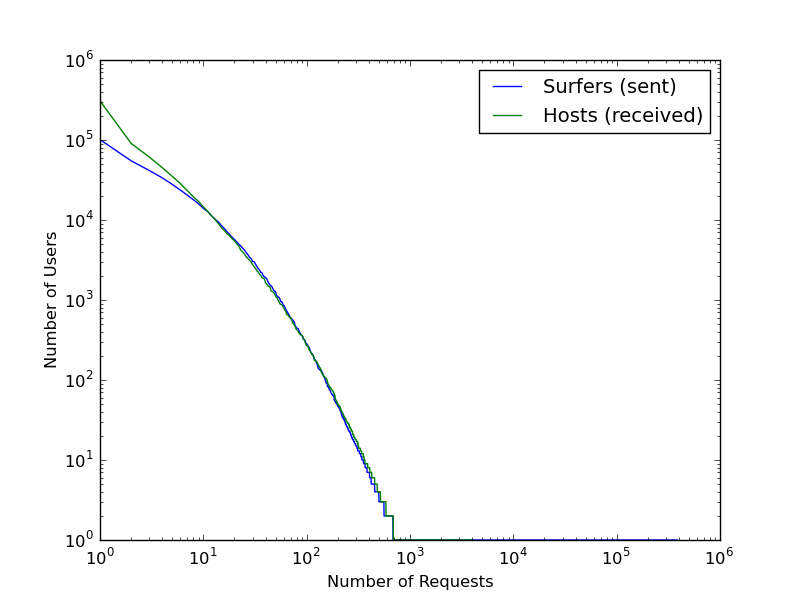
\includegraphics[width=1\linewidth]{figures/req_received_dist2.png}
\caption{Distribution of requests received by a host. \todo{Tobi: these numbers must be incorrect}}
\label{fig:requests_distribution}
\end{figure}

In the light of the described need of CouchSurfing, we focused on the evaluation from the host perspective, i.e. rejects are not as important (surfer's care about rejects) and assistance is particularly important when the host faces a lot of couchrequest at the same time (a large competitor set). Therefore, we look at all competitor sets that have a winner and group them by their cardinality. We compare our system against a random baseline, and several rule-based approaches that presumably resemble the system currently in use at Couchsurfing (e.g. ordering by the number of references or friends). We call these single-feature baselines. Unfortunately, the ranking algorithm currently deployed at CouchSurfing was not shared with us, yet. However, we were told that it is a simple rule-based approach that most likely involves the parameters mentioned above.

We use two different measures to evaluate performance: Prediction Accuracy (PA), and Average Normalized Winner Rank (ANWR). Prediction Accuracy is the fraction of correctly predicted winner's from several competitor sets (larger is better). Average Normalized Winner Rank is a more general measure that captures what position the actual winner has in our computed ranking/smaller is better) We normalize the rank to be between zero and number of competitors minus one. Note that a prediction only counts as a positive towards PA if it occured at the first place in the ranking. The ANWR is less strict in this case. \todo{maybe something mathematical here?}

We compute these two measure on the CouchSurfing Data that has 11 million couch request grouped into 5.5 million competitor sets. We split these competitor sets into a training, validation, and test set (60/20/20\%) in time to ensure that we do not look ahead into the future to make predictions easier. Please not that the state of the system we compute our features from lies ``in the future''. This can help but in some cases hurt as described below.

For a summary of the results see Figure \todo{put figure here tobi} which shows PA and ANWR on competitorsets of a certain minimum cardinality. One can observe that we consistently outperform the baselines by X-Y percent. For larger competitor sets the recommendation or ranking task becomes harder and performance drops. Especially in this regime, our algorithm supports hosts better in choosing the right couch surfer to accept. Due to the normalization the ANWR stays roughly constant. The average rank for the random baseline is 0.5 (``the middle''). Interestingly, some of the single-feature baselines do worse than the random baseline (e.g. the number of people that have vouched to you) even though one might think they would be helpful. The number of friends and the number of references performs better. Using our system, on average, a host needs to browse 39\% of the list compared to 46\% for the the second best ranking approach.

Why is this such a hard problem? First of all, notice that estimating probabilities including the possibility of rejection is much harder than just ranking of candidates due to the fact that rejectance might have nothing to do with the candidates themself or the hosts preference but may simply be dependent on the host's availability. This availability is hard to to infer automatically from the user's profile. For us it was impossible to capture this kind of time-dependent information because we were only supplied with the current state of the CouchSurfing database. Furthermore, note that this also means that we cannot know e.g. when two users became friends on the network. This can lead to interfering behavior. Assume that we know that host $h$ accepted surfer $s$ from  a competitor set $S$ and we know that they are friends. Our model infers that it this friendship might be \textit{the} critical and discriminative feature. However, $h$ and $s$ might not have been friends before the accepted couchrequest but only after they spent some time with each other. Similarly, our current model does not capture other temporal relationships such as whether host and surfer had been in contact before the actual request. We hypothesize that accurate modeling of this temporal structure in the data should improve performance significantly.




